\subsection{\TeX, eine DSL für Dokumente}

\TeX~ ist eine weit verbreitete Programmiersprache die speziell für die
Aufgaben eines Textsatzsystem erschaffen wurde. Daher kann man
\TeX~ auch als eine \emph{externe DSL} ansehen.
In diesem Abschnitt wird etwas auf
\TeX~ eingegangen, da insbesondere diese Programmiersprache als Inspiration
bzw. Vorbild dient.


\subsubsection{Herkunft und Grundlagen}

Der Name hat seinen Ursprung aus dem griechischen $\tau\epsilon\chi$,
welches auch die Wurzel für das englische Wort \emph{technology} ist.
$\tau\epsilon\chi$ bedeutet also Technologie, aber auch Kunst.
(\cite{tex-a}, Kapitel 1, Seite 1)

\TeX~ ist ein Dokumenten-Compiler, welcher dazu gedacht ist hochqualitativen
Textsatz zu erstellen, mit einem starken Fokus auf
Mathematik. \TeX82 ist in der Programmiersprache Pascal-H definiert
bzw. in WEB. (\cite{tex-b}, §1, Seite 1)

Die prototypische Entwicklung begann im Sommer 1977, Version 0 wurde
im September 1982 fertig gestellt, seit dem wurde TeX eingefroren
und seither wird nur noch an der Stabilität und Zuverlässigkeit
gearbeitet. (\cite{tex-b}, §2, Seite 2)

Es gibt etwa 300 \TeX~Kontrollsequenzen, sog. „Primitive“ welche das
Low-Level TeX bilden. Diese Primitiven sind atomisch und werden nicht weiter
in kleinere Funktionen zerlegt.
Zudem kommen noch etwa 600 weitere, aus Primitiven zusammengesetzte,
Kontrollsequenzen „plain \TeX“ dazu,
die zusammen mit den Primitiven das Standard-\TeX~bilden.
(\cite{tex-a}, Kapitel 3, Seite 9--11)

\TeX~ hat eine \emph{REPL}\footnote{REPL steht für read–eval–print loop,
eine interaktive Programmierumgebung. Scala besitzt auch eine REPL.
Dieser kann unter UNIX mit dem Befehl \lstinline|tex| aufgerufen werden.}
in welcher interaktive Programmiersitzungen abgehalten werden können,
wie z.B.:

\paragraph{Primitiv}

\begin{verbatim}
**\show\input
> \input=\input.
\end{verbatim}

\paragraph{Zusammengesetzte Kontrollsequenz, ein Makro}

\begin{verbatim}
**\show\TeX
> \TeX=macro:
->T\kern -.1667em\lower .5ex\hbox {E}\kern -.125emX.
\end{verbatim}

Viele Ligaturen\footnote{Ligaturen wie z.B. \lstinline|ff| zu ff}
werden von TeX als solche erkannt und direkt also solche
im resultierenden Dokument umgesetzt. Zudem können mit einer gewöhnlichen
Tastatur auch ungewöhnliche Zeichen gesetzt werden, so kann z.B. mit der
\lstinline|\ss| \TeX-Sequenz ein ß gesetzt werden, was dem Dokument
schöne Typographie bzw. Zeichen anderer Sprachen, mit lateinischen
Zeichen, erlaubt. (\cite{tex-a}, Kapitel 9, Seite 51--52)

Jedes einzelne Zeichen ist eine Box welche, aus Höhe, Breite, Tiefe und
einer Basisline besteht, diese Boxen können
zu größeren Einheiten „verklebt“ werden, so dass daraus schlussendlich
auch komplizierte Seiten-Layouts zusammengestellt werden können.
(\cite{tex-a}, Kapitel 11, Seite 63)

\begin{figure}[h!]
  \centering
    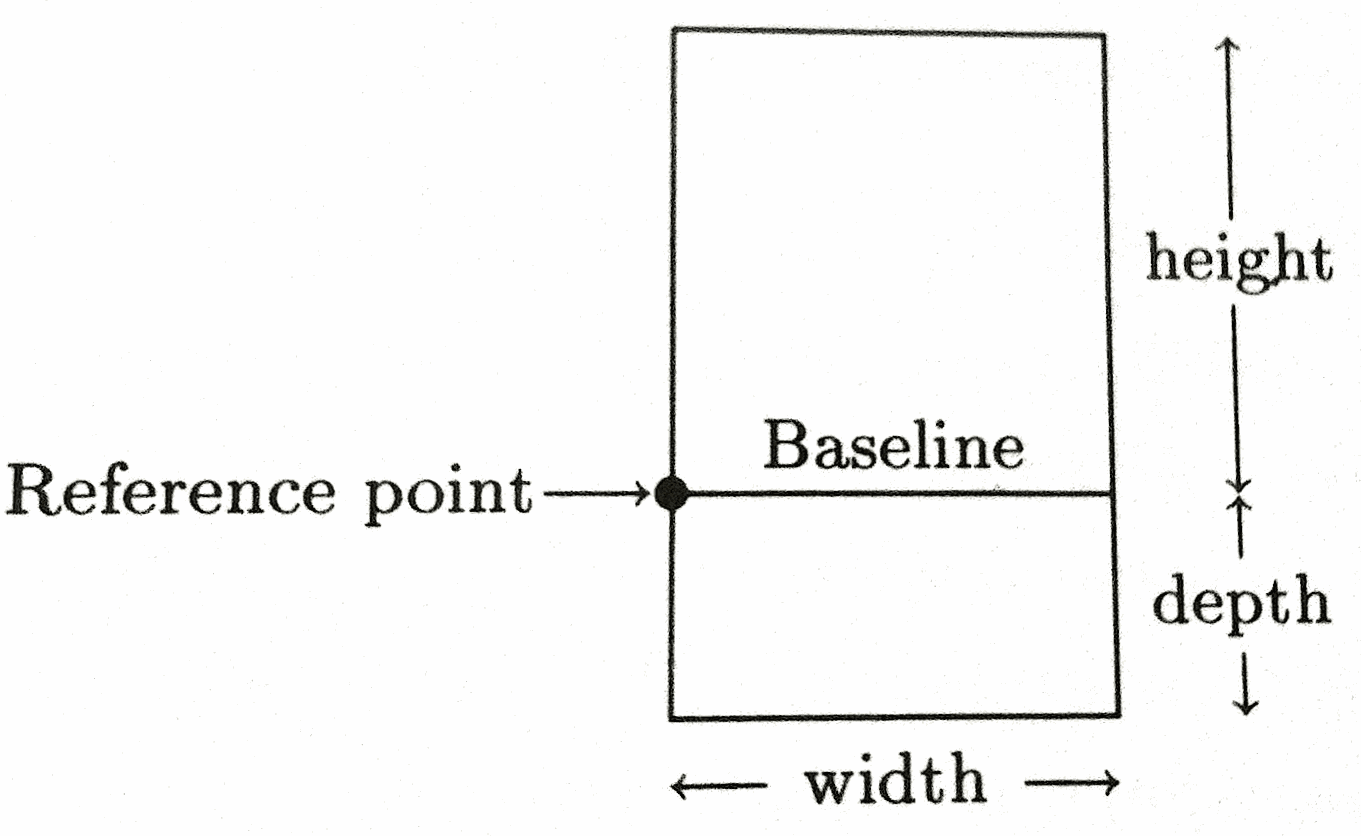
\includegraphics[width=0.5\textwidth]{figures/tex_box.png}
  \caption{\TeX~ Box für jedes einzelnes Zeichen.
           (\cite{tex-a}, Kapitel 11, Seite 63)}\label{fig-tex_box}
\end{figure}

\TeX~ kann einen Abschnitt in einzelne Zeilen herunterbrechen, so dass
der Benutzer sich nicht um diese Aufgabe kümmern muss. Es wird der beste
Weg gesucht, für den jeweiligen Abschnitt das „minimale Übel“ zu finden.
(\cite{tex-a}, Kapitel 14, Seite 91)
Die Methode die in TeX verwendet wird, geht auf Michael F. Plass
und Donald E. Knuth zurück. (\cite{tex-b}, §813, Seite 343)
Zudem ist ein Silbentrennungsalgorithmus enthalten, der auf
Frank M. Liang zurückgeht. (\cite{tex-b}, §919, Seite 386)

Das Dokument in einzelne Seiten zu unterteilen kann \TeX~ automatisch
vornehmen. Machmal ist es allerdings geschickter, wenn der Dokumentenersteller
mit etwas Handarbeit den Seitenumbruch selbst einstellt, um ein ideales
Ergebnis zu erzielen. (\cite{tex-a}, Kapitel 15, Seite 109)

\subsubsection{Fähigkeiten als Programmiersprache}

Mit den geschweiften Klammern \{ und \} sind die Gruppierungssymbole, so
dass Änderungen innerhalb einer Gruppe nicht auch Dinge außerhalb
verändern. (\cite{tex-a}, Kapitel 5, Seite 19)
Das Verhalten ist also gewohnt wie es in Programmiersprachen wie C,
Java oder Scala vorkommt.

Makros bzw. Definitionen ermöglichen es Abkürzungen für z.B. häufig
verwendete Kontrollsequenzen anzulegen, so dass insbesondere
der Quellcode übersichtlicher wird bzw. der Dokumentenersteller sich
Schreibarbeit sparen kann.

\begin{verbatim}
\def\xvec{(x_1,\ldodts,x_n)} --> \xvec
\end{verbatim}

TeX expandiert dann automatisch das Makro für den Benutzer.
So ist es sinnvoll wenn TeX-Benutzer ihre eigene kleine Bibliothek mit
Makros zusammenstellen, so dass sie diese in verschiedenen Dokumenten
wiederverwenden können. (\cite{tex-a}, Kapitel 20, Seite 199)
\LaTeX~ ist \emph{u.a.} eine sehr bekannte und beliebte
Bibliothekszusammenstellung\footnote{\url{http://www.latex-project.org}}.

\begin{verbatim}
\input macros  % Importiert aus macros.tex
\end{verbatim}

Parametrisierte Makros sind auch möglich, was TeX eine mächtige
Makroprogrammierfähigkeit verschafft:

\begin{verbatim}
\def\cs #1. #2\par{...}
\end{verbatim}

Wobei in diesem Beispiel nach Aufruf von \lstinline|\cs| Parameter
\lstinline|#1| so lange gilt,
bis \lstinline|". "| auftritt und Parameter \lstinline|#2|
bis \lstinline|'\par'| auftritt. (\cite{tex-a}, Kapitel 20, Seite 202)

Die Makros können auch rekursiv aufgebaut werden, so dass damit auch möglich ist
Schleifen (tail recursive) zu bilden.
(\cite{tex-a}, Kapitel 20, Seite 219)
TeX selbst bietet auch ein \lstinline|\loop...\repeat| Kommando an,
mit dessen Hilfe Schleifen gebildet werden können.
(\cite{tex-a}, Kapitel 20, Seite 217)


\paragraph{Einer Kontrollsequenz eine Bedeutung zuweisen:}

\begin{itemize}
  \item \lstinline|\font\cs=<font name>|
        (\lstinline|\cs| wird ein font identifier),
  \item \lstinline|\chardef\cs=<number>|
        (\lstinline|\cs| wird ein character code),
  \item \lstinline|\countdef\cs=<number>|
        (\lstinline|\cs| wird ein \lstinline|\count| register,
        was quasi einer int Variablen entspricht),
  \item \lstinline|\def\cs...{...}|
        (\lstinline|\cs| wird ein Macro),
  \item \lstinline|\let\cs=<token>|
        (\lstinline|\cs| bekommt die Bedeutung des Tonkens)
\end{itemize}

\paragraph{Beispiel}

\begin{verbatim}
\let\a=\macroname
\end{verbatim}

\lstinline|\a| wird zu \lstinline|\macroname| aufgelöst, quasi wie eine Referenz.
(\cite{tex-a}, Kapitel 20, Seite 206)


Makros können auch ihr Verhalten abhängig durch bestimmte Bedingungen
ändern, indem mit \lstinline|\if<condition><true text>\else<false text>\fi|
Bedingungen
aufgestellt werden. Es gibt verschiedene in TeX hart Codierte
\lstinline|<condition>|
wie z.B. \lstinline|\ifnum| zum Testen auf \lstinline|>, <, 0| eines count-Registers.
(\cite{tex-a}, Kapitel 20, Seite 207)
\TeX ~hat verschiedene if-Anweisungen wie \lstinline|\if|, \lstinline|\iftrue| oder \lstinline|\ifvoid| etc.,
diese Anweisungen sind fester Bestandteil der sprachlichen Grammatik.
(\cite{tex-a}, §487, Seite 197, §489, Seite 198)

\TeX~ unterstützt also Funktionsaufrufe in Form von Makros,
Verzweigungsentscheidungen
und rekursive Aufrufe bzw. Schleifen. Somit ist \TeX~ \emph{turing-vollständig.}

Auch hat TeX rudimentäre Eingabe/Ausgabe Fähigkeiten, indem es
bis zu 16 Dateien gleichzeitig öffnen und lesen kann, jedoch sind auch
diese Makros hart einkodiert wie z.B. \lstinline|\openin0=<filename>|.
Auch ist es möglich mit \lstinline|\message{...}| auf das Standard-Out zu schreiben
bzw. mit \lstinline|\read...to\varname| vom Standard-In zu lesen.
(\cite{tex-a}, Kapitel 20, Seite 217)

\subsubsection{Warum \TeX~ so aussieht, wie es aussieht}

Das Sprachdesign von \TeX~ ist auf Dokumentengenerierung ausgelegt, dies
bedingt, dass Zeichen bzw. Zeichenketten der Hauptbestandteil des Codes
sind. Der Benutzer will also so wenig wie möglich explizite Angaben über
Zeichenketten-Literale machen, daher fängt \emph{jeder Befehl} in \TeX~
mit einem \lstinline|\| an, zwar sehen die Befehle dann etwas gewöhnungsbedürftig
aus, aber daher kann alles andere als Zeichenkette vom Parser
wahrgenommen werden.

\TeX~ unterscheidet zwischen 16 Zeichenkategorien, um die Sprache zu parsen:

\begin{enumerate}
  \item Escape \lstinline|\|
  \item Gruppenbeginn \lstinline|{|
  \item Gruppenende \lstinline|}|
  \item Mahtemodus \$
  \item Alignment tab \lstinline|&|
  \item End of line \lstinline|<return>|
  \item Parameter \lstinline|#|
  \item Superscript \lstinline|^|
  \item Subscript \lstinline|_|
  \item Ignored character \lstinline|<null>|
  \item Space
  \item Letter \lstinline|A,...,z a,...,z|
  \item Other character (Keiner der anderen)
  \item Active character \lstinline|~|
  \item Kommentar \%
  \item Invalid \lstinline|<delete>|
\end{enumerate}

(\cite{tex-a}, Kapitel 7, Seite 37)

\subsubsection{Was \TeX~ generiert}

Hier ein kleines Basisskript, welches so in den REPL getippt werden kann und
eine gesetzte \lstinline|textput.dvi| Datei produziert:

\begin{verbatim}
**\relax
*Hello World!
*This is \TeX
*\end
\end{verbatim}

TeX verwendet internen immer den eigenen Zeichencode und konvertiert beispielsweise
\lstinline|'b'| immer in die \TeX-Sequenz \lstinline|\char98| um.
(\cite{tex-a}, Kapitel 8, Seite 43)

Das \emph{device-independent file format (DVI)} ist ein Stream aus
8-Bit bytes, welche eine Serie an
Maschinencode ähnliches Kommandos enthält, zur Zeichnung eines Dokuments.
\TeX~ liefert die Seiten in Form einer DVI-Datei aus.
(\cite{tex-b}, §583, Seite 234, §584, Seite 235, §592, Seite 244)

Die \TeX-Kontrollsequenzen sind auf Pascal Prozeduren abgebildet,
welche schlussendlich DVI-Dateien produzieren. Das bedeutet, dass der Generator
relativ fest verdrahtet und somit schwierig zu ändern ist.

\paragraph{Produktionsformat versus Auslieferungsformat}

\TeX~ stellt ein Konzept besonders klar dar: die \emph{Unterscheidung
zwischen Produktionsformat und Auslieferungsformat.} Diese Unterscheidung
wird von vielen Menschen nicht verstanden oder wahrgenommen; daher kommt
es immer mal wieder vor, dass Microsoft Word Dateien im E-Mail Anhang zu
finden sind.

Bei \TeX~ ist das Produktionsformat die Quellcode-Dateien und in neuerer
Zeit ist das Auslieferungsformat eine gesetzte PDF-Datei, welche auf jeder
Plattform gleich angezeigt wird und auch als Archivierungsformat tauglich
ist.
